\PassOptionsToPackage{table}{xcolor}
\documentclass[aspectratio=169,11pt]{beamer}

\usepackage{fontspec}
\usepackage{graphicx}
\usepackage{booktabs}
\usepackage{tabularx}
\usepackage{array}

\setsansfont[
  Path=template/forta/fonts/,
  Extension=.ttf,
  UprightFont=NeueHaasDisplayRoman,
  BoldFont=NeueHaasDisplayBold,
  ItalicFont=NeueHaasDisplayRomanItalic,
  BoldItalicFont=NeueHaasDisplayBoldItalic
]{NeueHaasDisplayRoman}

\setmainfont[
  Path=template/forta/fonts/,
  Extension=.ttf,
  UprightFont=NeueHaasTextRegular,
  BoldFont=NeueHaasTextBold
]{NeueHaasTextRegular}

\setmonofont[
  Path=template/generic/fonts/inconsolata/,
  Extension=.otf,
  UprightFont=Inconsolata-LGC,
  BoldFont=Inconsolata-LGC-Bold,
  ItalicFont=Inconsolata-LGC-Italic,
  BoldItalicFont=Inconsolata-LGC-BoldItalic
]{Inconsolata-LGC}

\definecolor{thesisred}{HTML}{C81919}
\definecolor{thesisdark}{HTML}{151515}
\definecolor{thesisgray}{HTML}{5A5A5A}
\definecolor{thesislight}{HTML}{F6F3EF}
\definecolor{thesisgreen}{HTML}{2E6F40}

\setbeamercolor{background canvas}{bg=white}
\setbeamercolor{normal text}{fg=thesisdark,bg=white}
\setbeamercolor{frametitle}{fg=thesisdark,bg=white}
\setbeamercolor{title}{fg=thesisdark}
\setbeamercolor{structure}{fg=thesisred}
\setbeamercolor{itemize item}{fg=thesisred}
\setbeamercolor{itemize subitem}{fg=thesisred}
\setbeamercolor{block title}{fg=white,bg=thesisred}
\setbeamercolor{block body}{fg=thesisdark,bg=thesislight}
\setbeamercolor{alertblock title}{fg=white,bg=thesisdark}
\setbeamercolor{alertblock body}{fg=thesisdark,bg=thesislight}
\setbeamercolor{footline}{fg=white,bg=thesisdark}

\setbeamertemplate{navigation symbols}{}
\setbeamertemplate{itemize item}{\raise0.2ex\hbox{\small$\blacksquare$}}
\setbeamertemplate{itemize subitem}{\raise0.2ex\hbox{\tiny$\blacksquare$}}

\setbeamersize{text margin left=0.75cm,text margin right=0.75cm}
\setbeamerfont{title}{size=\Huge,series=\bfseries}
\setbeamerfont{subtitle}{size=\Large}
\setbeamerfont{frametitle}{size=\LARGE,series=\bfseries}
\setbeamerfont{block title}{series=\bfseries}

\setbeamertemplate{footline}{%
  \leavevmode%
  \hbox{%
    \begin{beamercolorbox}[wd=.84\paperwidth,ht=3.1ex,dp=1.2ex,leftskip=0.8cm]{footline}%
      \usebeamerfont{footline}\insertshorttitle
    \end{beamercolorbox}%
    \begin{beamercolorbox}[wd=.16\paperwidth,ht=3.1ex,dp=1.2ex,center]{footline}%
      \usebeamerfont{footline}\insertframenumber/\inserttotalframenumber
    \end{beamercolorbox}%
  }%
}

\graphicspath{{images/}}

\title[Deep Program Induction for Personal Healthcare]{Deep Program Induction\\for Personal Healthcare}
\subtitle{Defense talk}
\author{Vadim Liventsev}
\institute{Eindhoven University of Technology}
\date{May 2026}

\newcommand{\takeaway}[1]{%
  \begin{alertblock}{Takeaway}
    #1
  \end{alertblock}
}

\begin{document}

\begin{frame}[plain]
  \vspace{0.4cm}
  {\color{thesisred}\rule{\linewidth}{4pt}}

  \vspace{0.8cm}
  {\usebeamerfont{title}\inserttitle\par}
  \vspace{0.35cm}
  {\usebeamerfont{subtitle}\color{thesisgray}\insertsubtitle\par}

  \vfill
  \begin{tabular}{@{}l@{}}
    \textbf{Vadim Liventsev}\\
    Eindhoven University of Technology\\
    \insertdate
  \end{tabular}

  \vspace{0.6cm}

  {\large\color{thesisgray}How can code-generating AI help build more transparent healthcare decision support?}
\end{frame}

\begin{frame}{Why This Topic Matters}
  \begin{columns}[T,totalwidth=\textwidth]
    \column{0.57\textwidth}
      \begin{itemize}
        \item Healthcare needs stronger decision support, but the cost of mistakes is unusually high.
        \item Black-box AI can be powerful, yet hard to audit, regulate, and trust in the clinic.
        \item Reinforcement learning could search for better treatment strategies, but we cannot safely learn them on real patients.
      \end{itemize}

    \column{0.39\textwidth}
      \begin{block}{Core challenge}
        We need learning systems that are both \textbf{capable} and \textbf{inspectable}, plus realistic ways to test them before deployment.
      \end{block}
  \end{columns}
\end{frame}

\begin{frame}{Research Goal}
  \begin{block}{Main objective of the thesis}
    Develop \textbf{program induction technology for health services based on deep learning}.
  \end{block}

  \vspace{0.3cm}

  \begin{itemize}
    \item Can we learn decision policies as \textbf{executable programs} rather than opaque weight matrices?
    \item Can those programs be \textbf{audited, improved, and reused} by humans and other AI systems?
    \item What kinds of \textbf{patient simulators} are needed to make this practical for healthcare?
  \end{itemize}

  \takeaway{The thesis tackles both halves of the problem: better code-generating methods and better healthcare testbeds.}
\end{frame}

\begin{frame}{How The Talk Follows The Thesis}
  \begin{tabularx}{\textwidth}{>{\raggedright\arraybackslash}p{0.18\textwidth} >{\raggedright\arraybackslash}p{0.18\textwidth} >{\raggedright\arraybackslash}p{0.26\textwidth} >{\raggedright\arraybackslash}p{0.22\textwidth}}
    \rowcolor{thesislight}
    \textbf{Introduction} & \textbf{Proposal} & \textbf{Program induction} & \textbf{Healthcare} \\
    Why code? & RLCEPS framework & BF++, neurogenetic, Tree2Tree, BOPTEST, SEIDR & Simulators survey, HeartPole, Auto-ALS, MIMIC-SEQ
  \end{tabularx}

  \vspace{0.6cm}

  \begin{itemize}
    \item First: why program induction is interesting for healthcare.
    \item Second: the thesis framework, \textbf{RLCEPS}.
    \item Third: methods contributions.
    \item Fourth: healthcare simulators and benchmarks.
    \item Finally: what this all adds up to.
  \end{itemize}
\end{frame}

\begin{frame}{What Is Deep Program Induction?}
  \begin{columns}[T,totalwidth=\textwidth]
    \column{0.54\textwidth}
      \begin{itemize}
        \item \textbf{Program synthesis}: automatically producing software from a specification.
        \item The specification can be text, input-output examples, or reward from an environment.
        \item In this thesis, the learned artifact is not just a model --- it is \textbf{code that can be run, tested, read, and edited}.
      \end{itemize}

      \vspace{0.2cm}
      \takeaway{Program induction treats executable code as the model representation.}

    \column{0.43\textwidth}
      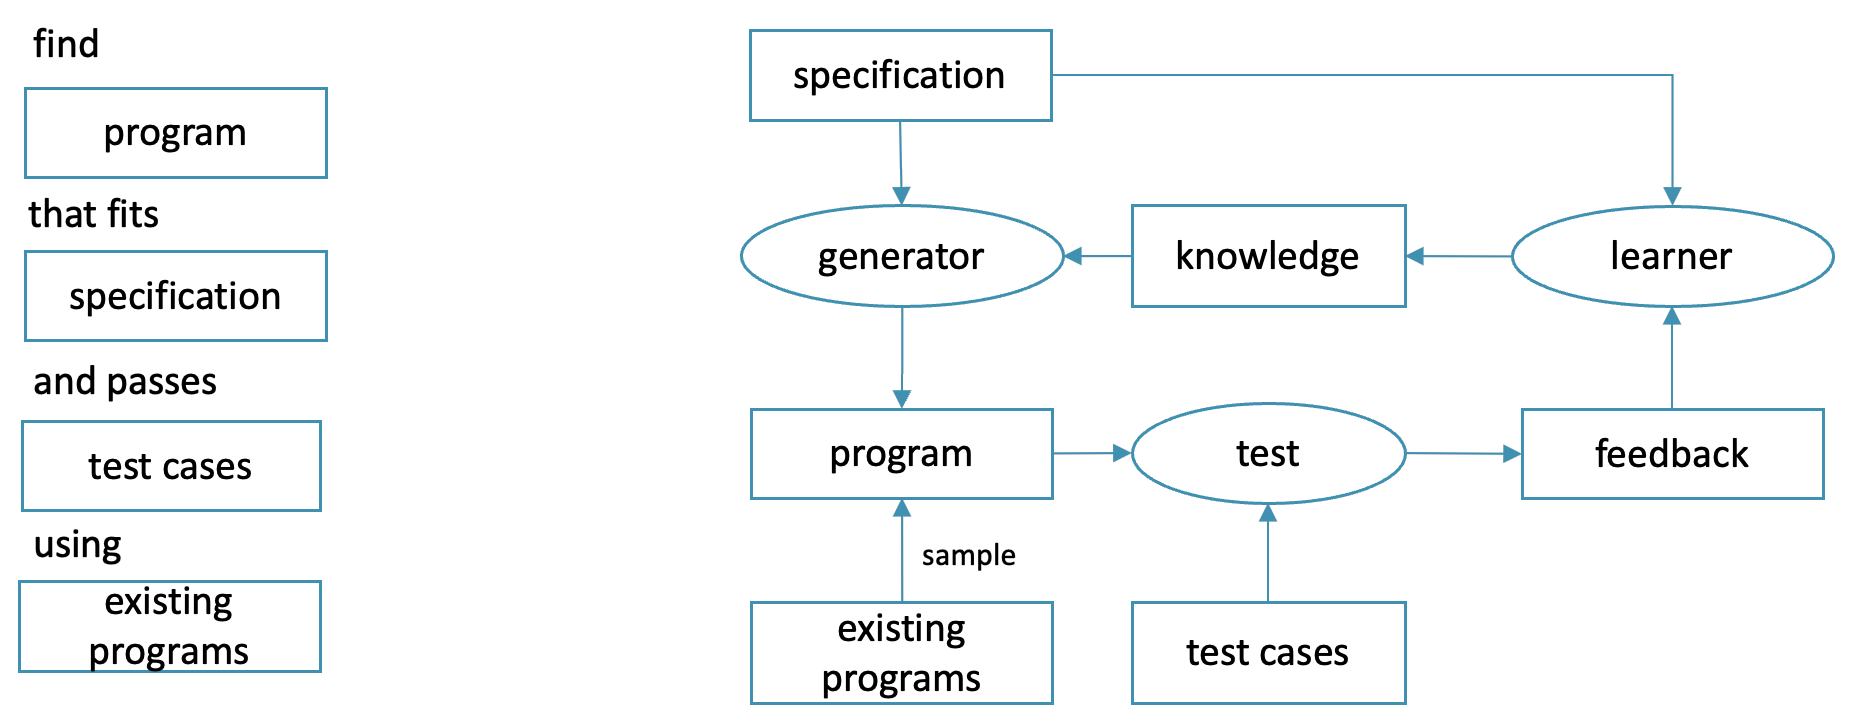
\includegraphics[width=\linewidth]{ap.png}
  \end{columns}
\end{frame}

\begin{frame}{Why Use Code Instead Of A Black Box?}
  \begin{columns}[T,totalwidth=\textwidth]
    \column{0.44\textwidth}
      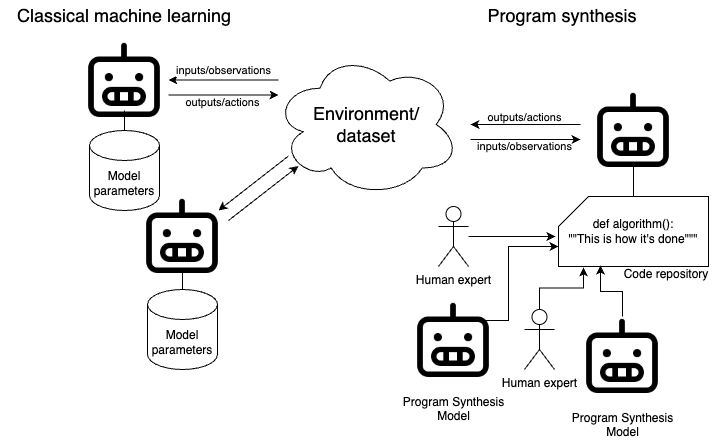
\includegraphics[width=\linewidth]{mlvsautocode.png}

    \column{0.52\textwidth}
      \begin{itemize}
        \item Programs are often \textbf{compact, fast, and expressive}.
        \item Existing expert knowledge can be \textbf{imported} as a starting program.
        \item The result can be \textbf{verified} before deployment and later \textbf{exported} back into human knowledge.
      \end{itemize}

      \vspace{0.25cm}
      \begin{block}{Why healthcare in particular?}
        Healthcare demands transparency, compliance, teamwork with clinicians, and strong protection against hidden failure modes.
      \end{block}
  \end{columns}
\end{frame}

\begin{frame}{Core Proposal: RLCEPS}
  \begin{columns}[T,totalwidth=\textwidth]
    \column{0.56\textwidth}
      \begin{itemize}
        \item Learn or construct a \textbf{patient simulator}.
        \item Search for a treatment policy represented as \textbf{executable code}.
        \item Evaluate candidate programs in simulation before any real-world use.
      \end{itemize}

      \vspace{0.25cm}
      \begin{block}{RLCEPS}
        \textbf{Reinforcement Learning from Code Execution Feedback in Patient Simulators}: the thesis framework for interpretable healthcare RL.
      \end{block}

    \column{0.40\textwidth}
      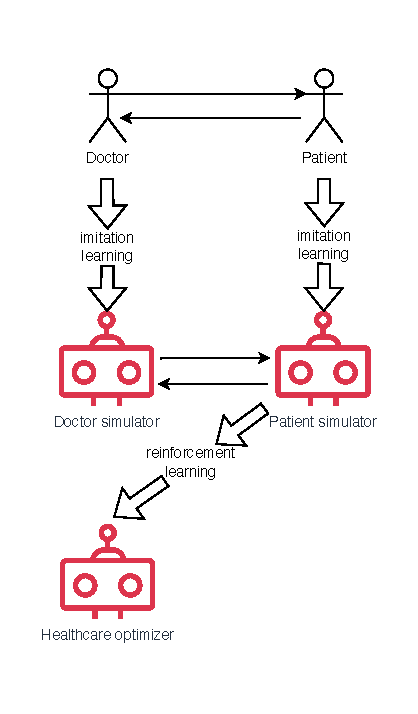
\includegraphics[width=\linewidth,height=0.52\textheight,keepaspectratio]{rlceps.pdf}
  \end{columns}
\end{frame}

\begin{frame}{Contributions At A Glance}
  \begin{columns}[T,totalwidth=\textwidth]
    \column{0.48\textwidth}
      \begin{block}{Program induction contributions}
        \begin{itemize}
          \item BF++
          \item Neurogenetic programming
          \item Tree variational autoencoder for code
          \item Iterative LLM programming in BOPTEST
          \item SEIDR multiagent framework
        \end{itemize}
      \end{block}

    \column{0.48\textwidth}
      \begin{block}{Healthcare contributions}
        \begin{itemize}
          \item Survey of patient simulators
          \item HeartPole sanity-check benchmark
          \item Auto-ALS emergency-care benchmark
          \item MIMIC-SEQ dataset for future simulators
        \end{itemize}
      \end{block}
  \end{columns}
\end{frame}

\begin{frame}{Part I: Closing The Methods Gap}
  \begin{block}{The thesis attacks three bottlenecks}
    \begin{enumerate}
      \item \textbf{Search space}: what programming language or representation should we search in?
      \item \textbf{Search algorithm}: neural, genetic, tree-based, or LLM-driven?
      \item \textbf{Feedback}: how do we turn execution results into better next candidates?
    \end{enumerate}
  \end{block}

  \vspace{0.3cm}

  \begin{itemize}
    \item Early chapters focus on constrained languages and hybrid search.
    \item Later chapters move to iterative large-language-model programming with tests in the loop.
  \end{itemize}
\end{frame}

\begin{frame}{BF++: A Tiny Language For Interpretable RL}
  \begin{columns}[T,totalwidth=\textwidth]
    \column{0.54\textwidth}
      \begin{itemize}
        \item BF++ is a domain-specific language designed to make reinforcement-learning policies easier to search as programs.
        \item A smaller language reduces the search space and keeps the resulting code readable.
        \item On classic control tasks, the method found functional solutions and sometimes came close to deep RL performance while staying explainable.
      \end{itemize}

      \takeaway{Constraining the language can make program search feasible without giving up interpretability.}

    \column{0.40\textwidth}
      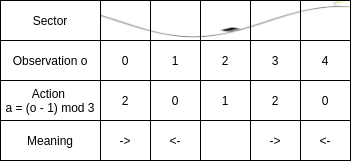
\includegraphics[width=\linewidth]{MountainCarWinner.png}
  \end{columns}
\end{frame}

\begin{frame}{Hybrid And Structure-Aware Search}
  \begin{columns}[T,totalwidth=\textwidth]
    \column{0.48\textwidth}
      \begin{block}{Neurogenetic programming}
        \begin{itemize}
          \item Combines neural developers with genetic operators.
          \item Hybrid teams outperformed purely neural or purely genetic variants on benchmark tasks.
        \end{itemize}
      \end{block}

    \column{0.48\textwidth}
      \begin{block}{Tree variational autoencoder}
        \begin{itemize}
          \item Represents code as abstract syntax trees, not just token strings.
          \item Produced better low-dimensional code representations than sequence-to-sequence baselines.
        \end{itemize}
      \end{block}
  \end{columns}

  \vspace{0.2cm}
  \centering
  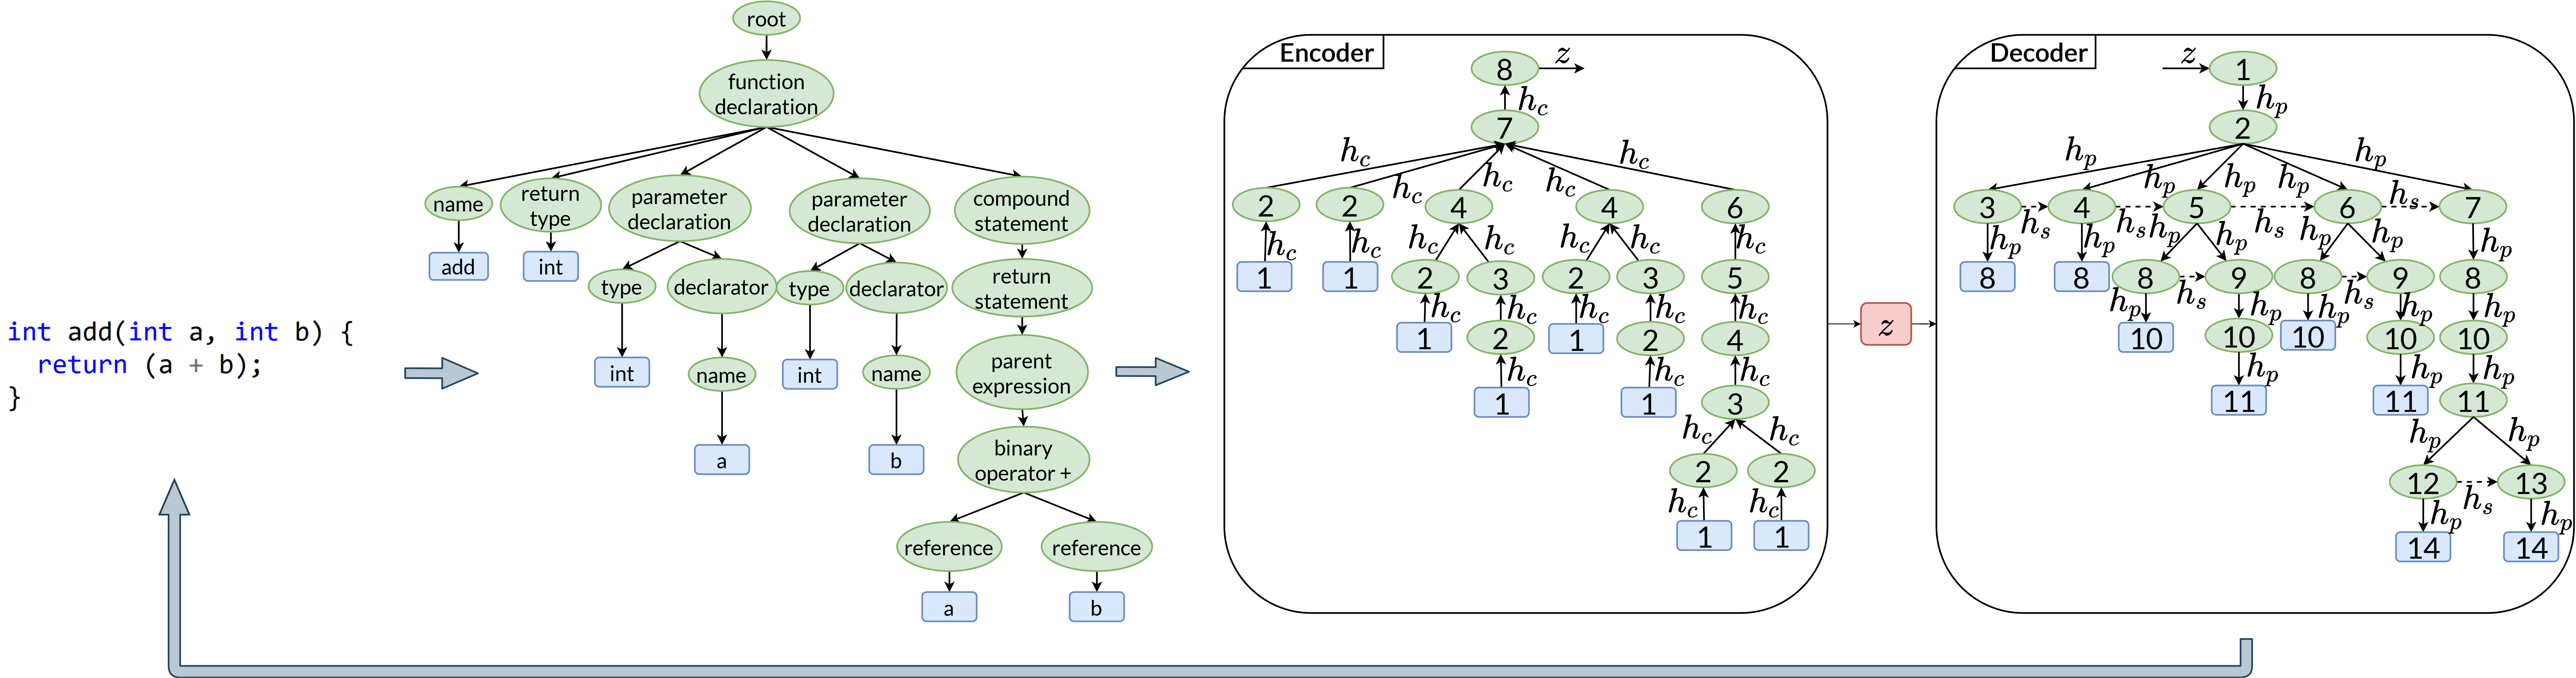
\includegraphics[width=0.34\linewidth]{tree2treeLSTM2.png}
\end{frame}

\begin{frame}{LLMs Work Better When They Iterate}
  \begin{block}{From BOPTEST to a general recipe}
    One-shot prompting is not enough for difficult control tasks. The thesis shows that a stronger pattern is:
  \end{block}

  \vspace{0.25cm}
  \centering
  {\Large \textbf{Synthesize} $\rightarrow$ \textbf{Execute} $\rightarrow$ \textbf{Analyze errors} $\rightarrow$ \textbf{Revise}}

  \vspace{0.35cm}

  \begin{itemize}
    \item In BOPTEST building control, iterative refinement produced meaningful controllers where direct prompting struggled.
    \item This insight grows into the most mature method in the thesis: \textbf{SEIDR}.
  \end{itemize}
\end{frame}

\begin{frame}{SEIDR: Synthesize, Execute, Instruct, Debug, Rank}
  \begin{columns}[T,totalwidth=\textwidth]
    \column{0.57\textwidth}
      \begin{itemize}
        \item SEIDR turns test failures into structured feedback and new code candidates.
        \item It balances \textbf{repairing promising programs} against \textbf{replacing bad ones}.
        \item On standard program-synthesis benchmarks it reaches state-of-the-art or near-state-of-the-art results.
      \end{itemize}

      \vspace{0.2cm}
      \begin{block}{Headline results}
        \begin{itemize}
          \item PSB2: \textbf{19/25} solved in initial experiments.
          \item HumanEval-C++ pass@100: \textbf{78.5\%} with GPT-3.5, \textbf{84.2\%} with Llama 3.
        \end{itemize}
      \end{block}

    \column{0.39\textwidth}
      \begin{tabular}{@{}ll@{}}
        \toprule
        \textbf{S} & Synthesize \\
        \textbf{E} & Execute \\
        \textbf{I} & Instruct \\
        \textbf{D} & Debug \\
        \textbf{R} & Rank \\
        \bottomrule
      \end{tabular}
  \end{columns}
\end{frame}

\begin{frame}{Program Induction: Main Lessons}
  \begin{block}{What Part I suggests}
    \begin{itemize}
      \item Reinforcement learning from code execution feedback is viable.
      \item The strongest systems are usually \textbf{hybrids}: symbolic, neural, evolutionary, and LLM-based ideas working together.
      \item Testing, debugging, and iteration matter at least as much as raw model size.
    \end{itemize}
  \end{block}

  \takeaway{By the midpoint of the thesis, we have a credible program-induction engine for healthcare settings --- but it still needs the right simulators.}
\end{frame}

\begin{frame}{Patient Simulators: Promise And Pitfalls}
  \begin{columns}[T,totalwidth=\textwidth]
    \column{0.48\textwidth}
      
\includegraphics[width=\linewidth]{sim.png}

    \column{0.48\textwidth}
      
\includegraphics[width=\linewidth]{pseudosim.png}
  \end{columns}

  \vspace{0.25cm}

  \begin{itemize}
    \item A simulator can be a \textbf{patient model} or a \textbf{benchmark}; these are not the same role.
    \item Many healthcare simulators are limited by small datasets, sampling bias, or confirmation bias.
    \item A biased simulator may be unsafe for clinical recommendations, but still valuable as a benchmark for comparing learning methods.
  \end{itemize}
\end{frame}

\begin{frame}{HeartPole: A Transparent Sanity Check}
  \begin{columns}[T,totalwidth=\textwidth]
    \column{0.48\textwidth}
      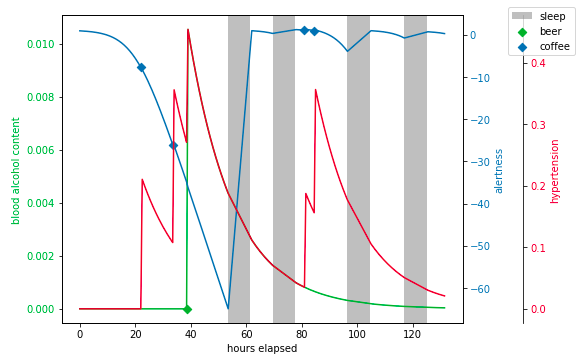
\includegraphics[width=\linewidth]{heartpole_example.png}

    \column{0.48\textwidth}
      \begin{itemize}
        \item HeartPole is intentionally simple and not clinically realistic.
        \item Its purpose is to make behavior easy to inspect while still requiring non-trivial long-term planning.
        \item Result: deep RL achieved the best raw score, but synthesized programs were competitive and much easier to read.
      \end{itemize}

      \vspace{0.2cm}
      \begin{block}{Why it matters}
        It is a clean sanity check: can interpretable program synthesis learn sensible behavior at all?
      \end{block}
  \end{columns}
\end{frame}

\begin{frame}{Auto-ALS: A Hard Emergency-Care Benchmark}
  \begin{columns}[T,totalwidth=\textwidth]
    \column{0.44\textwidth}
      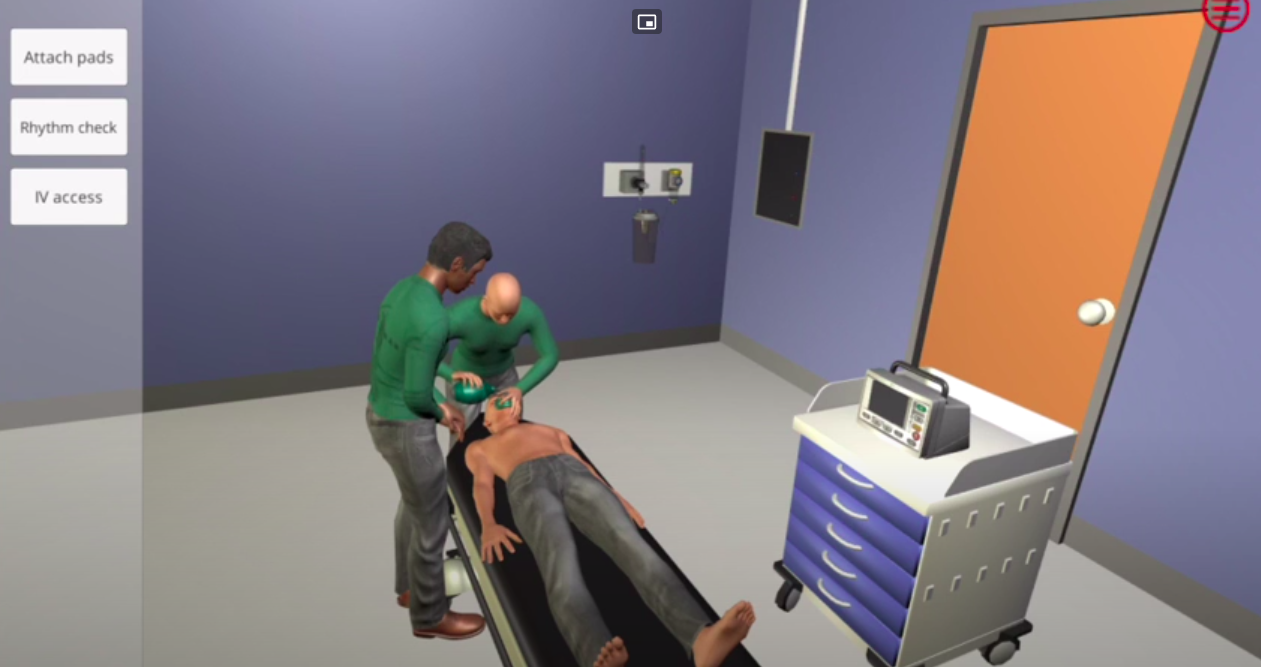
\includegraphics[width=\linewidth]{Virtu-ALS.png}

    \column{0.52\textwidth}
      \begin{itemize}
        \item Auto-ALS is derived from a didactic simulator for ABCDE emergency assessment.
        \item It is useful because the intended protocol is known, so we can compare learned behavior against expert expectations.
        \item Result: SEIDR made fewer blunders than PPO, but \textbf{neither method reliably stabilized the patient}.
      \end{itemize}

      \vspace{0.2cm}
      \takeaway{Auto-ALS remains unsolved and becomes a stress test for future healthcare RL methods.}
  \end{columns}
\end{frame}

\begin{frame}{MIMIC-SEQ: Toward Data-Driven Patient Simulators}
  \begin{columns}[T,totalwidth=\textwidth]
    \column{0.47\textwidth}
      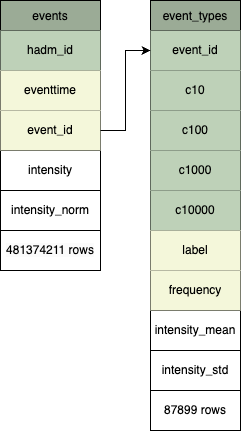
\includegraphics[width=\linewidth,height=0.46\textheight,keepaspectratio]{mimicseq.png}

    \column{0.49\textwidth}
      \begin{itemize}
        \item MIMIC-SEQ restructures MIMIC-IV intensive-care records as event sequences.
        \item It defines a standardized prediction task for future healthcare foundation models.
        \item Long term, it supports a larger and less confirmation-biased simulator than handcrafted educational environments.
      \end{itemize}

      \vspace{0.2cm}
      \begin{block}{Role in the thesis}
        MIMIC-SEQ bridges proof-of-concept benchmarks and scalable patient simulation.
      \end{block}
  \end{columns}
\end{frame}

\begin{frame}{What The Thesis Shows}
  \begin{itemize}
    \item Program induction is a plausible route to \textbf{transparent decision support} in healthcare.
    \item The best path is not purely symbolic or purely neural: it is \textbf{hybrid}.
    \item Progress on healthcare AI needs better \textbf{simulators and benchmarks}, not just better learning algorithms.
    \item With the right simulator, SEIDR-style methods can compete strongly and sometimes outperform traditional RL baselines while remaining interpretable.
  \end{itemize}

  \vspace{0.3cm}

  \takeaway{The thesis is a proof of concept for \textbf{programmatically interpretable reinforcement learning in healthcare} --- promising, but not finished.}
\end{frame}

\begin{frame}{Future Work And Questions}
  \begin{block}{Most important next steps}
    \begin{itemize}
      \item Better neurosymbolic representations for code.
      \item Intermediate pretraining curricula specialized for clinical programming and protocols.
      \item Turning clinical protocols into executable form.
      \item Scaling data-driven simulators and RLCEPS experiments.
    \end{itemize}
  \end{block}

  \vfill

  \centering
  {\Huge \textbf{Thank you}}\\[0.25cm]
  {\Large Questions?}
\end{frame}

\end{document}
